\section{Implementation}
\subsection{Simulated Network}

The network of our simulation is designed to give a real-time nature to the data transfer between the Tennessee Eastman(TE) physical simulation and the TE Controller. Both the controller and simulation are written in Matlab and connected to our network with the OMNeTBridge Class. 


\subsection{Controller}



\subsubsection{Actuator}

The actuator acts as a server which receives an update packet from the controller, grabs its appropriate data from the controller OMNeTBridge and then passes it to the correct function. 

\subsubsection{Sensor}


The Sensor is a relatively simple module that sends an update signal based on a timer. This is to model the refresh rate of most sensors. We have assumed that all sensors and network controllable and are able to tirelessly connect to a local access point via 802.11 Wireless LAN. 

These modules send a TCP packet to a known IP address which in turn triggers the controller to update. This is a non-ideal method of updating as it does not allow correct implementation of attacking the data on the network. Ideally INET's TCP packets would allow us to send data to them, however as some modules are currently implemented deep copies are not done of messages or inappropriate casts are used. Future work should be planned to modify these modules or find a more correct
implementation of INET messages that allow custom data fields to be created and sent. 


\subsection{MATLAB Simulation}
  Our MATLAB both simulated a system and a controler of the
  Tennessee Eastman problem, and used a custom packet interface
  between C++ and MATLAB as explained below.

\subsubsection{Tennessee Eastman}
  We buit a custom simplified Tennesee Eastman model in MATLAB.  
  This was based off of a preexisting FORTRAN model, but was
  reimplemented in MATLAB for ease of use and reduced complexity 
  \citation{Ricker}.  Our model contains variable vectors, an
  input vector, a state vector, and an output vector. Then by 
  using the equations provided in Ricker\citation{Ricker}, the
  simulation simply takes in the input vector from OMNeT++, and
  outputs the output vector, which includes the sensor data, to
  OMNeT++ via the MATLAB bridge.

  On the other side of the network, we also implemented a 
  controller in MATLAB for the Tennesee Eastman system.  This
  used steady state calculations to determine the optimal controls.
  The controller would input the output vector from the Tennessee
  Eastman system via the MATLAB bridge, and output a set of input
  vectors to be transmitted across the network into the MATLAB
  bridge.

\subsection{C++ to MATLAB Bridge}

\begin{figure*}
        \centering
		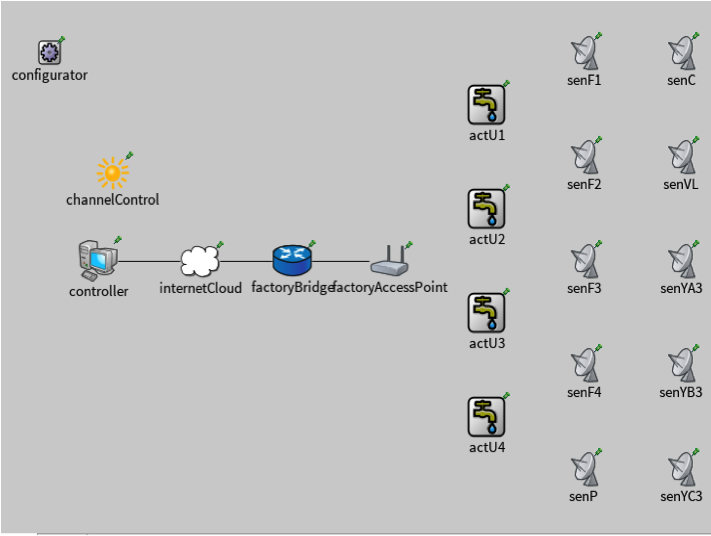
\includegraphics[width=0.8\textwidth]{figs/network.png}
        \caption{Network Diagram.}
        \label{fig:network}        
\end{figure*}
